\documentclass[a4paper]{article}
\usepackage[utf8]{inputenc}
\usepackage[spanish, es-tabla]{babel}
\usepackage[margin=0.7in]{geometry}
\usepackage{amsmath}
\usepackage{amsfonts}
\usepackage{amssymb}
\usepackage{xcolor}

\usepackage{float}
\usepackage{graphicx}
\graphicspath{ {./Imagenes/} }

\usepackage[american voltages,american currents]{circuitikz}

\usepackage{fancyhdr}

\usepackage{units} 

\pagestyle{fancy}
\fancyhf{}
%\lhead{23.09 Física Electrónica}
\rhead{Bertachini, Lambertucci, Londero, Mechoulam, Musich}
\rfoot{Página \thepage}


\begin{document}

%%%%%%%%%%%%%%%%%%%%%%%%%%%%%%%%%%%%%%%%%%%%%%%%%%%%%%%%%%%%%%%%%%%%%%%%% 
%								CARATULA								%
%%%%%%%%%%%%%%%%%%%%%%%%%%%%%%%%%%%%%%%%%%%%%%%%%%%%%%%%%%%%%%%%%%%%%%%%% 

\begin{titlepage}
\newcommand{\HRule}{\rule{\linewidth}{0.5mm}}
\center
\mbox{\textsc{\LARGE \bfseries {Instituto Tecnológico de Buenos Aires}}}\\[1.5cm]
\textsc{\Large 23.09 Física Electrónica}\\[0.5cm]

\HRule \\[0.6cm]
{ \Huge \bfseries Trabajo práctico N$^{\circ}$1}\\[0.4cm] 
\HRule \\[1.5cm]


{\large

\emph{Grupo 5}\\
\vspace{3px}

\begin{tabular}{lr}
\textsc{Bertachini}, Germán  & 58750 \\ 	
\textsc{Lambertucci}, Guido Erinque  & 58009 \\
\textsc{Londero Bonaparte}, Tomás Guillermo  & 58150 \\
\textsc{Mechoulam}, Alan  &  58438\\
\textsc{Musich}, Francisco  & 58124 \\

\end{tabular}

\vspace{20px}

\emph{Profesores}\\
\vspace{3px}
\textsc{Baez}, Eduardo Diocles\\ 	
\textsc{Cesaretti}, Juan Manuel\\ 
\textsc{Douthat}, Analia Elizabeth\\ 
\textsc{Gardella}, Pablo Jesús\\ 	

\vspace{100px}

\begin{tabular}{ll}

Presentado: & 24/06/19\\

\end{tabular}

}

\vfill

\end{titlepage}


%%%%%%%%%%%%%%%%%%%%%%%%%%%%%%%%%%%%%%%%%%%%%%%%%%%%%%%%%%%%%%%%%%%%%%%%% 
%								INFORME									%
%%%%%%%%%%%%%%%%%%%%%%%%%%%%%%%%%%%%%%%%%%%%%%%%%%%%%%%%%%%%%%%%%%%%%%%%%

\section*{Introducción}

En el trabajo presente se llevó adelante el estudio de distintos tipos de diodos y circuitos, con el objetivo de llevar a la práctica la teoría estudiada en clase y contrastar los datos obtenidos con los modelos teóricos.

\section*{Desarrollo de la Experiencia}

\subsection*{Medición de Diodos}

Se realizó la medición de las curvas características de tres diodos distintos: Rectificador 1N4148, Diodo Zener 12V y LED rojo de 5mm en ese orden respectivamente. Los diodos fueron conectados de la forma presentada en el circuito (\ref{circ:1}).

\begin{figure}[H]
\begin{center}
\begin{circuitikz}
\draw
	(4,0)	to (0,0)
	(0,1.5)	to [sV,v_=$V$]	(0,0)
	(0,1.5)	to [R, l_=$ 470 \ \Omega $]	(4,1.5)
	(4,0)	to [Do, l_=Diodo analizado]	(4,1.5)
;\end{circuitikz}
\end{center}
\caption{Circuito utilizado para medir los diodos.}
\label{circ:1}
\end{figure}

Haciendo uso de multímetros para el diodo rectificador y el diodo zener, y el osciloscopio para el LED, se observaron los comportamientos de cada diodo a ciertas tensiones para posteriormente graficar las curvas características correspondiente a cada uno.

Se realizó una superposición de las curvas de valores medidos en el laboratorio con las curvas teóricas realizadas con los datos proporcionados por el fabricante de cada dispositivo. Al costado de cada gráfico se muestra la curva obtenida mediante la simulación del circuito con el uso de \texttt{ltspice}.

\begin{figure}[H]
	\centering
	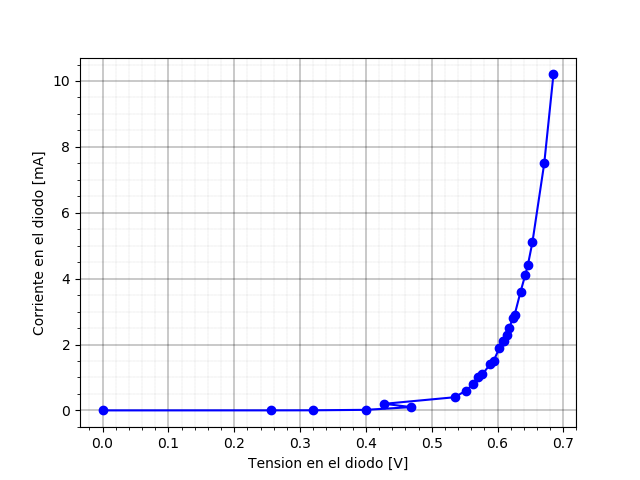
\includegraphics[width=0.7\textwidth]{CurvaDiodoRectificador.png}
	\caption{Superposición de las curva característica medida/simulada del diodo rectificador 1N4148.}
	\label{fig:diodorect}
\end{figure}

\begin{figure}[H]
	\centering
	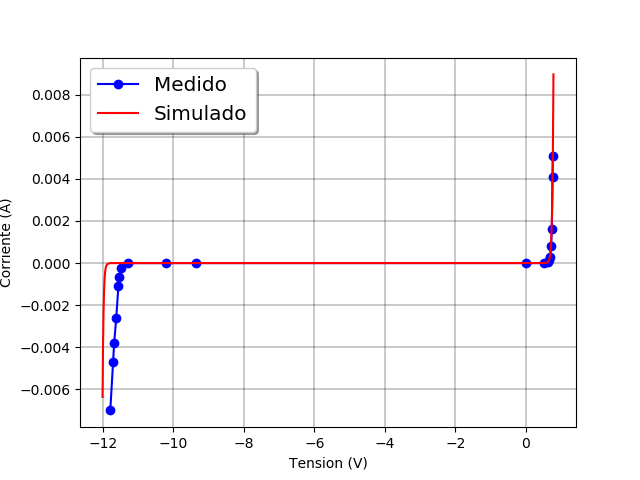
\includegraphics[width=0.7\textwidth]{CurvaZenerEntera.png}
	\caption{Superposición de las curva característica medida/simulada del diodo zener.}
	\label{fig:diodozen}
\end{figure}

\begin{figure}[H]
	\centering
	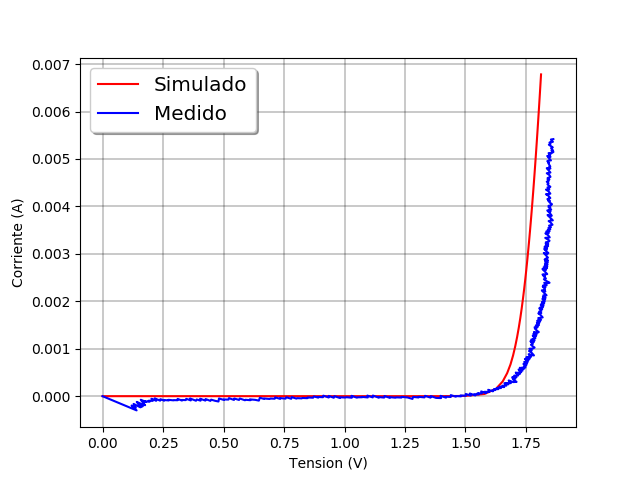
\includegraphics[width=0.7\textwidth]{CurvaDiodosLed.png}
	\caption{Superposición de las curva característica medida/simulada del diodo LED.}
	\label{fig:diodoled}
\end{figure}

\textcolor{red}{HACER ANALISIS}

\subsection*{Simulación de Circuito con Transistor}

Se procedió a realizar la simulación del siguiente circuito en \texttt{ltspice}:
\begin{figure}[H]
	\centering
	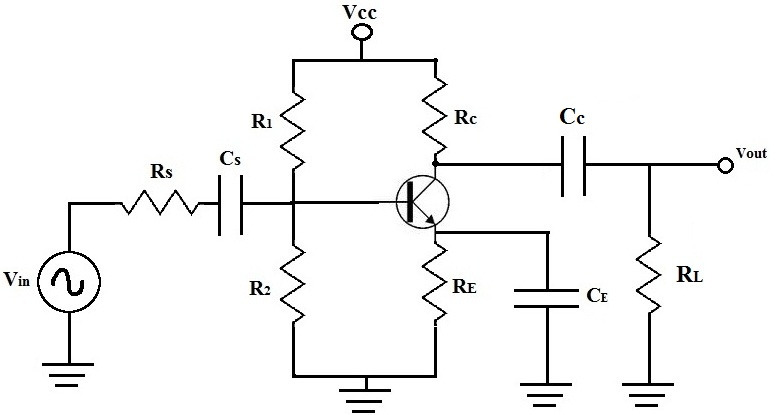
\includegraphics[width=0.6 \textwidth]{commonEmitter.jpg}	
	\caption{Circuito provisto por la catedra.}
	\label{fig:cmnemitnpn}

\end{figure}

Analizando la función transferencia de tensión de este, se observa que la transferencia para la zona constante es de $44,36 \ dB$, siendo de $43,19 \ dB$ el valor obtenido en simulación.

\begin{figure}[H]
	\centering
	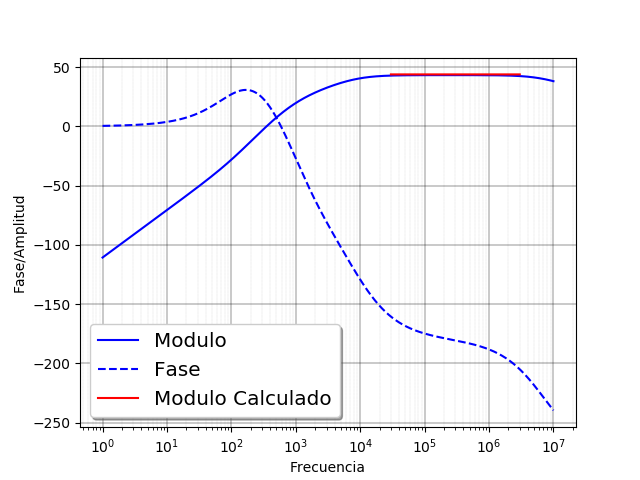
\includegraphics[width=0.9\textwidth]{RtaF2.png}	
	\caption{Diagrama de BODE para el circuito dado siendo la curva de mayor trazo el diagrama de amplitud.}
	\label{fig:bode}
\end{figure}

\subsection*{Simulación del Circuito con Diodo}

Se quizo analizar la respuesta en frecuencia del circuito en la figura (\ref{circ:3}) con \texttt{ltspice}, obteniendo el diagrama de Bode en la figura (\ref{fig:rtaf}).

\begin{figure}[H]
\begin{center}
\begin{circuitikz}[scale=1.5]
\draw

	(0,0)	to (4,0)
	(0,1.5)	to [sV,v_=$AC$]	(0,0)
	(0,2.5)	to [V,v_=$DC$]	(0,1.5)
	(0,2.5)	to[R,l=$R_G$,a=$50\Omega$] (2,2.5)
	(0,2.5)	to[R,l=$R_G$] (2,2.5)
	(2,2.5)	to[R,l=$R$,a=$100K\Omega$] 	(4,2.5)
	(2,2.5)	to[R,l=$R$] 	(4,2.5)
	(4,0)	to [Do, l_=D1N4007]	(4,2.5)
;\end{circuitikz}
\end{center}
\caption{Respuesta en frecuencia del 1N4007.}
\label{circ:3}
\end{figure}

\begin{figure}[H]
	\centering
	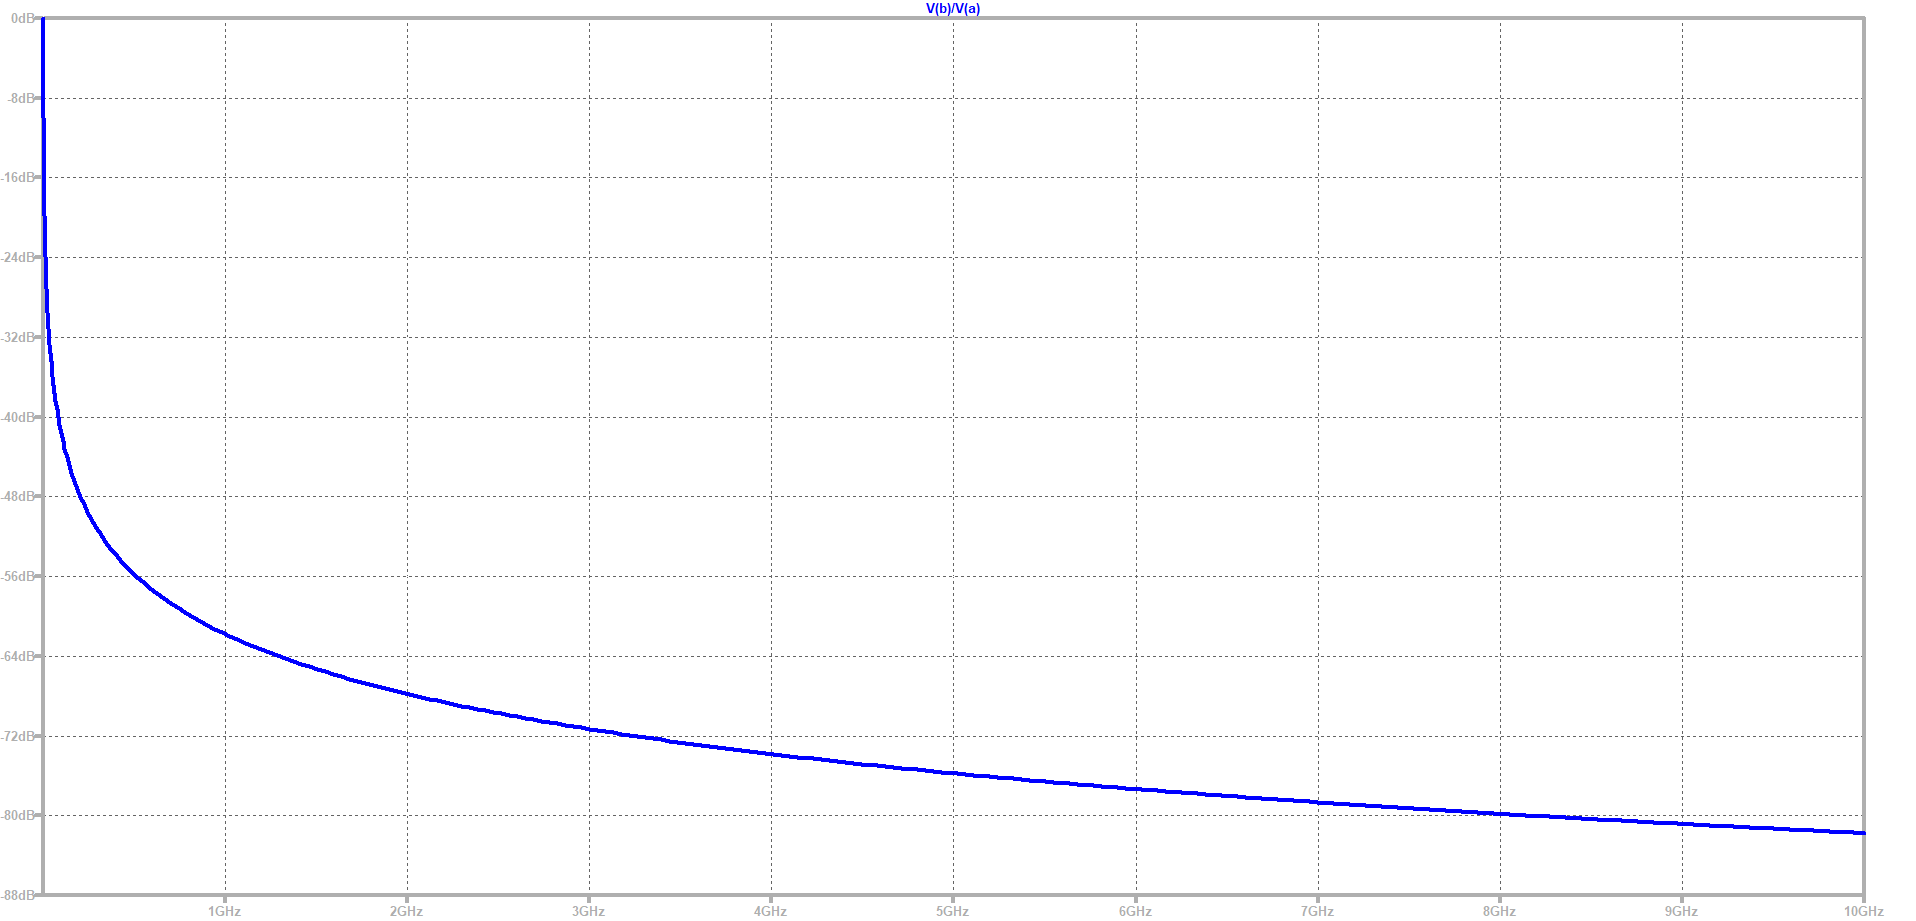
\includegraphics[width=0.9\textwidth]{RtaF3.png}	
	\caption{Respuesta en frecuencia del diodo D1N4007 siendo la curva de mayor trazo el diagrama de amplitud.}
	\label{fig:rtaf}
\end{figure}

Se puede observar como el comportamiento de la respuesta en frecuencia es similar a la de un filtro pasabajos de primer orden. Esto indica que el diodo puede ser asociado a un elemento capacitivo.
Para obtener la frecuencia de corte, se toma el valor de la frecuencia cuando la ganancia es de -3dB, obteniendo $f_c \approx 800KHz$.

Para caracterizar al diodo por su circuito equivalente, se utilizó un capacitor en paralelo con una resistencia. El valor de la resistencia fue obtenida por medio de la simulación la cual es de $1T\Omega$. La capacitancia del circuito equivalente puede ser calculada como $c=\frac{1}{2\pi R f_c}$, obteniendo un valor de $1,989pF$. Este valor es similar al obtenido mediante el uso de \texttt{ltspice}, $1,95pF$ respectivamente. Ambos valores se encuentran en el orden de la capacitancia declarada por el fabricante de $4pF$.

Finalmente, la figura (\ref{circ:4}) muestra el circuito equivalente del diodo 1N4007.

\begin{figure}[H]
\begin{center}\begin{circuitikz}[scale=1.8]\draw
(0,1) to[V, l=$DC$,a=$5V$] (0,2)
(0,0) to[sV, l=$AC$,a=$1V$] (0,1)
(0,2) to[R,l=$R_G$]  (2,2)
(2,2) to[R,l=$100K\Omega$] (3,2)
(3,2) -- (5,2)
(3.5,2) to[R,l=$R_D$,a=$1T\Omega$] (3.5,0)
(5,0)	to [C, l=$C$,a=1.95pF]	(5,2)
(0,0) -- (5,0);
\end{circuitikz} 
\end{center}
\caption{Circuito equivalente del diodo.}
\label{circ:4}
\end{figure}

\section*{Conclusión}

\textcolor{red}{COMPARAR CON MODELO TEORICO!!}
\textcolor{red}{NO REPETIR MEDICIONES ES INADMISIBLE}
\textcolor{red}{NO EXPLICADO COMO SACAMOS LA GANANCIA}
\textcolor{red}{QUE MODELO DE TRANSISTOR USAMOS? COMO SACAMOS RPI R0 GM?? CONSIDERAMOS CAP PARASITA?? PUNTO Q?}
\textcolor{red}{REEMPLAZAR DIODO SOLO POR UN CAP ESTA MAL.}

Los resultados obtenidos al estudiar los tres primeros diodos se corresponden con los resultados esperados. Se observan pequeñas incongruencias en los gráficos, como por ejemplo en el gráfico (\ref{fig:diodorect}), que son atribuidos a cambios de escala de los instrumentos durante el análisis.

Luego se comprobó que, la función transferencia del segundo análisis, es acorde a la real, dejando pasar las frecuencias altas, acorde a lo esperado.

Por último, la respuesta en frecuencia del último punto mostró que un diodo conectado de esa forma se puede asociar a un capacitor. Esto se sustenta en que la capacitancia declarada por el fabricante es similar a la obtenida mediante un proceso de simulación.


\end{document}

